
%----------------------------------------------------------------------------------------
%	PART
%----------------------------------------------------------------------------------------


\part{Capítulo ocho}
\graphicspath{ {img/ch7/}, {img/} }

%----------------------------------------------------------------------------------------
%	CHAPTER 8
%----------------------------------------------------------------------------------------



%----------------------------------------------------------------------------------------
%	PART
%----------------------------------------------------------------------------------------


\chapter{Formulación de funciones financieras en Excel}

\section{Fórmulas del capítulo/Herramienta Excel}

\vspace{2mm}

\begin{center}
\begin{tabular}{ |p{8cm}| p{5cm}|}
\hline 
\rowcolor{orange!50}
\begin{center}\textbf{Nombre} \end{center}  & \begin{center} \textbf{Función Financiera en Excel} \end{center}  \\ \hline

Equivalencia de tasas periódicas &  TASA(m;;-1;1+i)\\\hline 

Tasa interés nominal anual vencida & TASA.NOMINAL(i;m) \\ \hline

Tasa interés periódica año vencido & INT.EFECTIVO(j;m) \\ \hline

Valor futuro & VF(i;n;;VA,0)\\ \hline 

Valor presente & VA(i;n;;VF,0)\\ \hline 

Valor presente serie uniforme vencida & VNA(i;R1;R2;R3;...) \\ \hline  

Valor futuro serie uniforme vencida &  VF(i;n;;VA,0)\\ \hline

Valor futuro serie uniforme anticipada & VF(i;n;;VA,1)\\ \hline 

Valor presente serie perpetua vencida & VA(i;n;R;0) \\ \hline

Valor presente gradiente aritmético & VNA(i;R1;R2;R3;...) \\ \hline

Valor presente gradiente geométrico & VNA(i;R1;R2;R3;...) \\ \hline

Valor cuota serie uniforme vencida & PAGO(i;n;P;F;0) \\ \hline

Valor cuota serie uniforme anticipada & PAGO(i;n;P;F;1) \\ \hline

Ecuación de valor & Función Buscar Objetivo\\ \hline

\end{tabular}
\end{center}

\clearpage

\section{Introducción}

En este capítulo veremos la forma de resolver ejercicios de Ingeniería Económica mediante el uso del ordenador, más específicamente usando el programa de Excel, mediante la implementación de las funciones financieras que este nos brinda, para esto es importante consultar la Guía para resolver ejercicios de Ingeniería Económica a partir de Excel financiero y el uso de funciones financieras en Excel presentes en el inicio de la guía ya que este ofrecerá la metodología que debe ser aplicada para la correcta resolución de los ejercicios, además de presentar en esta las funciones que pueden ser aplicadas dando una explicación de estas y mostrando donde pueden ser aplicadas. 
\\

Es importante resaltar las ventajas que ofrece la resolución de los ejercicios por este método: \\

\begin{itemize}
\item Eficiencia en cuanto a la resolución de los ejercicios es mayor.\\
\item Se reduce la fuente del error que se puede llegar a obtener en el ejercicio ya que no es necesario la aplicación de cálculos a mano o en calculadora ya que todo es realizado por Excel.\\
\item Mejora la presentación del ejercicio.\\
\item Permite realizar un análisis de sensibilidad que por otro método no es posible.\\

\end{itemize}

Para mostrar las ventajas que posee el uso de Excel a continuación se mostraran diversos ejemplos sobre los diferentes temas tomados de los capítulos 2, 4, 5, 6 y 7 presentes en la Guía de Ingeniería Económica.

\section{Ejemplos}

\textbf{Ejemplo 1}\\

Tomado del Capítulo 2, ejercicio número 3.

\vspace{2mm}

¿Qué capital debo invertir hoy para poder retirar un millón de pesos dentro de 18 meses suponiendo que el capital invertido gana el 28\% nominal anual semestre vencido?
\\\\
\textbf{Solución:}\\

\textbf{a}. Declaración de variables\\

	
	    $F=\$1'000.000$\\
	$	n=3 psv 
		\\
		j=28\% nasv
		\\
		i=14\% psv
		\\
		$F=\$1'000.000$\\
	$	$P=\$?$
	
\\

\clearpage

\textbf{b}.Tabla flujo de caja
\\

\begin{spacing}{0.1}
\begin{center}
\begin{tabular}{ |p{3.5cm}| p{3cm}|}
\hline 

\begin{center}\textbf{Periodo (psv) } \end{center}  & \begin{center} \textbf{Flujo} \end{center}  \\ \hline

\begin{center} 0 \end{center}   &  \begin{center} - \end{center}\\\hline

\begin{center}1 \end{center}    &  \begin{center} \$- \end{center} \\ \hline

\begin{center}2 \end{center}    &  \begin{center} \$- \end{center} \\ \hline 

\begin{center}3 \end{center}    & \begin{center} \$1.000.000,00 \end{center}  \\ \hline


\end{tabular}
\end{center}
\end{spacing}
\\ \\

\vspace{2mm}
\vspace{2mm}
 
\textbf{c}. Aplicación de funciones.
 \\
 
Se aplicará la función VA de la siguiente forma:     
 
 \begin{center}
	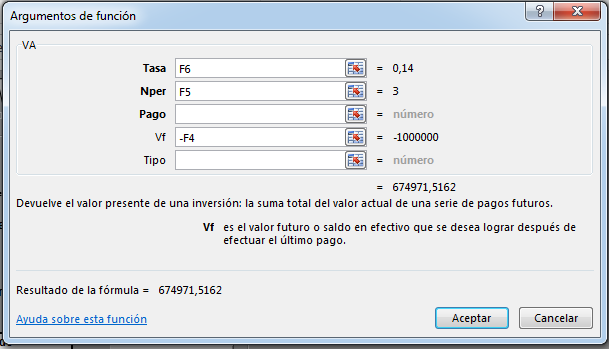
\includegraphics[height=5.4cm]{img/ch8/8_1.png}
\end{center}

=VA(F6;F5;;-F4) con referencia en la hoja de Excel de la declaración de variables.
\\ 
\vspace{2mm}

\textbf{d}. Respuesta

\vspace{2mm}

El monto es de \$ 674.971,52. 

\vspace{2mm}

\textbf{e}. Gráfica

\vspace{2mm}

No es necesaria la realización de una gráfica para este ejercicio.

\vspace{2mm}

\textbf{Ejemplo 2}\\

Tomado del Capítulo 2, ejercicio número 18.

\vspace{2mm}

Dado el  208\% p(3a)v hallar una tasa periódica equivalente para p(2a)v
\\\\
\textbf{Solución:}
\vspace{2mm}

\textbf{a}. Declaración de variables\\

	
	    
	$	m=3/2 p(2a)v 
		\\
		i1=208\% p(3a)v 
		\\
		i2=?\% p(2a)v
		\\
		$
	\\

\textbf{b}.Conversión de tasas
\vspace{2mm}

	$	m=3/2 p(2a)v 
		\\
		i1=208\% p(3a)v 
		\\
		i2=111,69\% p(2a)v
		\\
		$
\vspace{1mm}

\textbf{c}. Aplicación de funciones.
 \\
 
Se aplicará la función TASA de la siguiente forma:     
 
 \begin{center}
	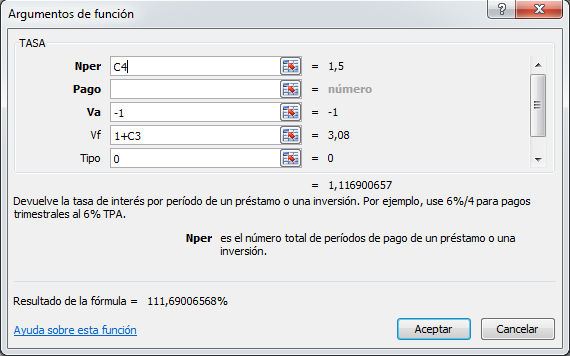
\includegraphics[height=5.4cm]{img/ch8/8_12.png}
\end{center}

=TASA(C4;;-1;1+C3) con referencia en la hoja de Excel de la declaración de variables.

\vspace{2mm}

\textbf{d}. Respuesta

\vspace{2mm}

La tasa es del 111,69\% período 2 años vencido 

\vspace{2mm}

\textbf{e}. Gráfica\\
No es necesaria la realización de una gráfica para este ejercicio.

\vspace{2mm}

\textbf{Ejemplo 3}\\

Tomado del Capítulo 2, ejercicio número 24

\vspace{2mm}

Una persona tiene dos deudas una de \$25.000 pagadera en 3 meses y otra de \$40.000 pagadera en 7 meses. Si desea cambiar la forma de cancelarlas mediante dos pagos iguales de \$X cada uno con vencimiento en 5 meses y 12 meses respectivamente, determinar el valor de los pagos suponiendo una tasa del 36\% nominal anual mes vencido.

\vspace{2mm}
\textbf{Solución:}\\

\textbf{a}. Declaración de variables\\


Deuda Inicial 

	    $D1=\$25.000,00?$
	    \\
	    $	n=3 pmv
	    \\
	     $D2=\$40.000,00?$
	    \\
	    $	n=7 pmv
	    \\
Deuda Equivalente 

	   $	n1=5 pmv $
	    \\
	    $	n2=10 pmv 
	    \\
		j=36,0\% namv
		\\
		i=3,0\% pmv
		\\
		
$

\textbf{b}. Tabla flujo de caja
\begin{spacing}{1.1}
    \begin{center}
        \begin{tabular}{|p{4cm}|p{4cm}|p{4cm}|}
        \hline 
            \textbf{Periodo} & \textbf{Deuda Inicial} & \textbf{Deuda Equivalente} \\ \hline                       
       
            0 & \$  &\$  \\ \hline
            1 & \$ &\$  \\ \hline
            2 & \$ & \$  \\ \hline
            3 & \$25.000,00  & \$ \\ \hline
            4 & \$  &\$  \\ \hline
            5 & \$ &\$0  \\ \hline
            6 & \$ & \$ \\ \hline
            7 & \$40.000,00  & \$ \\ \hline
            8 & \$&\$   \\ \hline
            9 & \$ &\$  \\ \hline
            10 & \$ & \$ \\ \hline
            11 & \$  & \$ \\ \hline
            12 & \$  & \$0 \\ \hline    

 
\end{tabular}
\end{center}
\end{spacing}

\textbf{c}. Aplicación de funciones.
 \\
 
Se aplicará la función VA de la siguiente forma:     
 
 \begin{center}
	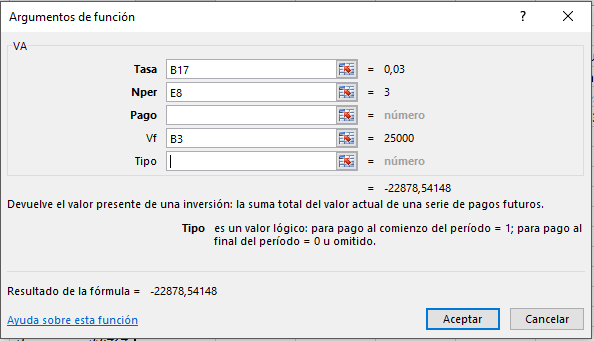
\includegraphics[height=5.4cm]{img/ch8/8_2.png}
\end{center}

Esta función se aplicará de la siguiente forma en las dos celdas donde se desee obtener el Valor presente de las deudas originales y de las deudas equivalentes.

\vspace{2mm}

=-VA(B17;E8;0;F8)-VA(B17;E12;0;F12) y en =-VA(B17;E10;0;G10)-VA(B17;E17;0;G17)

\vspace{2mm}

Luego se aplicará la formula Función Objetivo de la siguiente forma

\\
 \begin{center}
	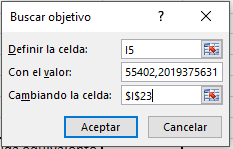
\includegraphics[height=5.4cm]{img/ch8/8_3.png}
\end{center}
\\ 
\textbf{d}. Respuesta

\vspace{2mm}


\begin{spacing}{1.1}
    \begin{center}
        \begin{tabular}{|p{4cm}|p{4cm}|p{4cm}|}
        \hline 
            \textbf{Periodo} & \textbf{Deuda Inicial} & \textbf{Deuda Equivalente} \\ \hline                        

           
            0 & \$  &\$  \\ \hline
            1 & \$ &\$  \\ \hline
            2 & \$ & \$  \\ \hline
            3 & \$25.000,00  & \$ \\ \hline
            4 & \$  &\$  \\ \hline
            5 & \$ &\$35.424,00  \\ \hline
            6 & \$ & \$ \\ \hline
            7 & \$40.000,00  & \$ \\ \hline
            8 & \$&\$   \\ \hline
            9 & \$ &\$  \\ \hline
            10 & \$ & \$ \\ \hline
            11 & \$  & \$ \\ \hline
            12 & \$  & \$35.424,00 \\ \hline    

 
\end{tabular}
\end{center}
\end{spacing}
Debe realizar dos pagos con el valor de \$35.423,66 cada uno.
\vspace{2mm}

\textbf{e}. Gráfica

\vspace{2mm}

No es necesaria la realización de una gráfica para este ejercicio.
\\\\
\textbf{Ejemplo 4}\\

Tomado del Capítulo 4, ejemplo número 2

\vspace{2mm}

Un documento estipula pagos trimestrales de \$80.000 durante 6 años. Si este documento se cancela con un solo pago de:
a) VP = \$? al principio; con una tasa del 32\% nominal anual año vencido.
b) VF = \$? al final, con una tasa del 32\% nominal anual año vencido.

\vspace{2mm}

\textbf{Solución:}
\vspace{2mm}

\textbf{a}. Declaración de variables\\

\\

	
	    $R=\$80.000,00$\\
	$	n=24 ptv 
		\\
		i=8,00\% ptv
		\\
		$	$P=\$?$
	
\\

\textbf{b}.Tabla flujo de caja
\\

\vspace{2mm}


\begin{spacing}{1.1}
    \begin{center}
        \begin{tabular}{|p{4cm}|p{4cm}|}
        \hline 
            \textbf{Periodo (ptv)} & \textbf{Flujo}  \\ \hline                        

           
            0 & \$ -  \\ \hline
            1 & \$ 80.000,00  \\ \hline
            2 & \$ 80.000,00   \\ \hline
            3 & \$80.000,00   \\ \hline
            4 & \$  80.000,00 \\ \hline
            5 & \$80.000,00   \\ \hline
            6 & \$ 80.000,00 \\ \hline
            7 & \$80.000,00   \\ \hline
            8 & \$80.000,00 \\ \hline
            9 & \$ 80.000,00 \\ \hline
            10 & \$ 80.000,00 \\ \hline
            11 & \$  80.000,00  \\ \hline
            12 & \$  80.000,00  \\ \hline    
 
\end{tabular}
\end{center}
\begin{center} Hasta 24 ptv \end{center}
\end{spacing}



\textbf{c}. Aplicación de funciones.
 \\
 
Se aplicará la función VA de la siguiente forma:     
 
 \begin{center}
	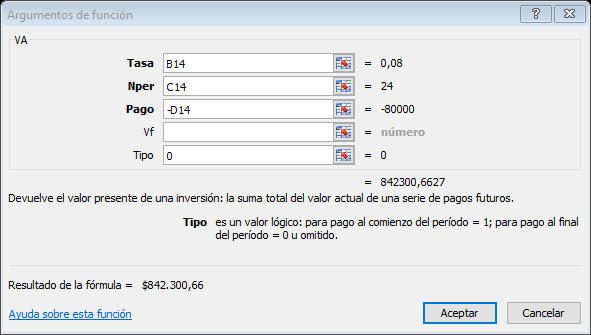
\includegraphics[height=5.4cm]{img/ch8/8_4.png}
\end{center}

=VA(B14;C14;-D14;;0) con referencia en la hoja de Excel usada para el ejercicio
\\
 \begin{center}
	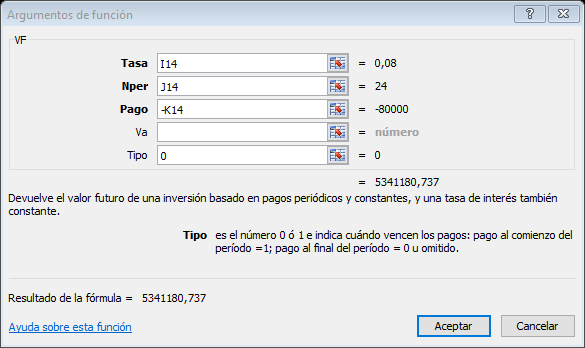
\includegraphics[height=5.4cm]{img/ch8/8_5.png}
\end{center}
=VF(I14;J14;-K14;;0) con referencia en la hoja de Excel usada para el ejercicio

\vspace{2mm}

\textbf{d}. Respuesta

\vspace{2mm}

El valor presente es VP = \$842.300,66 y el valor futuro es VF = \$5.341.180,74

\vspace{2mm}

\textbf{e}. Gráfica


\ \begin{center}
	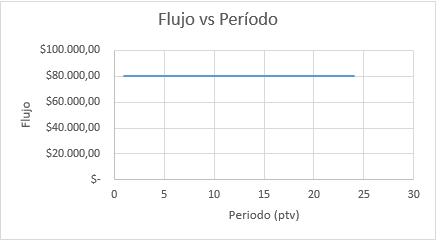
\includegraphics[height=5.4cm]{img/ch8/8_6.png}
\end{center}

\textbf{Ejemplo 5}\\

Tomado del Capítulo 4, ejercicio número 1

\vspace{2mm}

Hallar el monto y el valor presente de 20 pagos de \$2.000 cada uno, suponga una tasa del 18\% período año vencido.

\vspace{2mm}

\textbf{Solución:}

\vspace{2mm}

\textbf{a}. Declaración de variables\\

	    $R=\$2.000,00$\\
	$	n=20 pav 
		\\
		i=18\% pav $
		\\
		$F=\$?$
		\\
		$P=\$?$
		\\
	
	\\
	
	\clearpage

\textbf{b}.Tabla flujo de caja
\\

\begin{spacing}{0.1}
\begin{center}
\begin{tabular}{ |p{3.5cm}| p{3cm}|}
\hline 

\begin{center}\textbf{Periodo (psv) } \end{center}  & \begin{center} \textbf{Flujo} \end{center}  \\ \hline

\begin{center} 0 \end{center}   &  \begin{center} - \end{center}\\\hline

\begin{center}1 \end{center}    &  \begin{center} \$2.000,00\end{center} \\ \hline

\begin{center}2 \end{center}    &  \begin{center} \$2.000,00\end{center} \\ \hline 

\begin{center}3 \end{center}    & \begin{center} \$2.000,00 \end{center}  \\ \hline

\begin{center}4 \end{center}    & \begin{center} \$2.000,00 \end{center}  \\ \hline

\begin{center}5 \end{center}    & \begin{center} \$2.000,00 \end{center}  \\ \hline

\begin{center}6 \end{center}    & \begin{center} \$2.000,00 \end{center}  \\ \hline

\begin{center}7 \end{center}    & \begin{center} \$2.000,00 \end{center}  \\ \hline

\begin{center}8 \end{center}    & \begin{center} \$2.000,00 \end{center}  \\ \hline
\end{tabular}

\end{center}
\end{spacing}

\begin{center} Hasta 20 psv \end{center}

\textbf{c}. Aplicación de funciones.
 \\
 
Se aplicará la función VA de la siguiente forma:     
 
 \begin{center}
	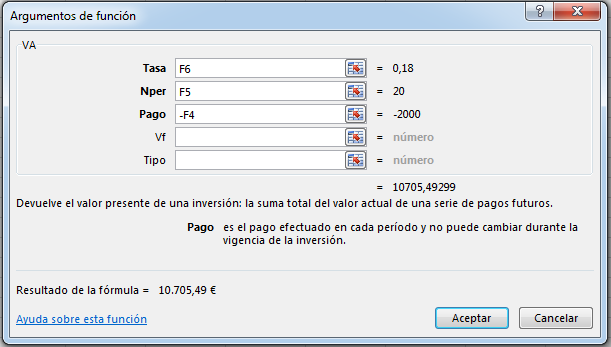
\includegraphics[height=5.4cm]{img/ch8/8_7.png}
\end{center}

\clearpage

=VA(F6;F5;-F4) con referencia en la hoja de Excel usada para el ejercicio.

\\
 \begin{center}
	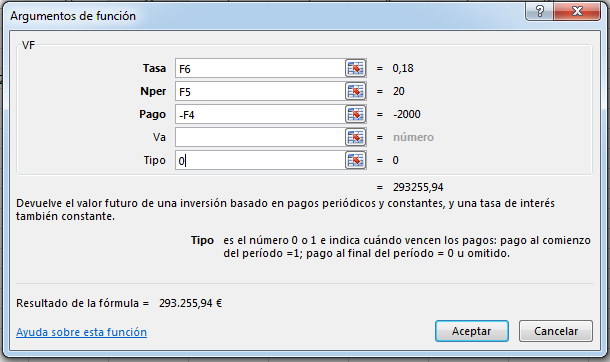
\includegraphics[height=5.4cm]{img/ch8/8_8.png}
\end{center}

=VF(F6;F5;-F4;;0) con referencia en la hoja de Excel usada para el ejercicio.

\vspace{2mm}

\textbf{d}. Respuesta

\vspace{2mm}

El valor presente VP = \$ 10.705,49 y el valor futuro es VF = \$ 293.3255,94.
\\\\
\textbf{e}. Gráfica
\begin{center}
	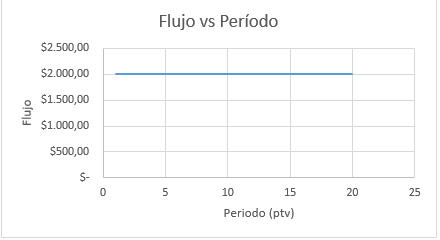
\includegraphics[height=5.4cm]{img/ch8/8_9.png}
\end{center}

\textbf{Ejemplo 6}\\

Tomado del Capítulo 4, ejercicio número 2

\vspace{2mm}

Para la compra de un automóvil que vale \$6.000.000,00; se exige una cuota inicial del 40\% y el resto se cancela en 36 cuotas mensuales, ¿a cuánto ascenderá la cuota, si lo intereses son del 3.5\% período mes vencido?

\vspace{2mm}

\textbf{Solución:}
\vspace{2mm}

\textbf{a}. Declaración de variables\\

	    $P=\$6.000.000,00?$
	    \\
	    $	n=36 pmv 
	    \\
		i=3,5\% pmv
		\\
		Cuota inicial = 40\%P $\\
		$R=\$?$\\
		
\clearpage

\textbf{b}.Tabla flujo de caja
\\

\begin{spacing}{0.1}
\begin{center}
\begin{tabular}{ |p{3.5cm}| p{3cm}|}
\hline 

\begin{center}\textbf{Periodo (psv) } \end{center}  & \begin{center} \textbf{Flujo} \end{center}  \\ \hline

\begin{center} 0 \end{center}   &  \begin{center} - \end{center}\\\hline

\begin{center}1 \end{center}    &  \begin{center} \$?\end{center} \\ \hline

\begin{center}2 \end{center}    &  \begin{center} \$?\end{center} \\ \hline 

\begin{center}3 \end{center}    & \begin{center} \$?\end{center}  \\ \hline

\begin{center}4 \end{center}    & \begin{center} \$? \end{center}  \\ \hline

\begin{center}5 \end{center}    & \begin{center} \$? \end{center}  \\ \hline

\begin{center}6 \end{center}    & \begin{center} \$? \end{center}  \\ \hline

\begin{center}7 \end{center}    & \begin{center} \$? \end{center}  \\ \hline
\begin{center}8 \end{center}    & \begin{center} \$? \end{center} \\ \hline
\end{tabular}
\end{center}
\end{spacing}
\\
\begin{center}Hasta el período 36 psv \end{center}

\textbf{c}. Aplicación de funciones.
 \\
 
Se aplicará la función PAGO de la siguiente forma:     
 
 \begin{center}
	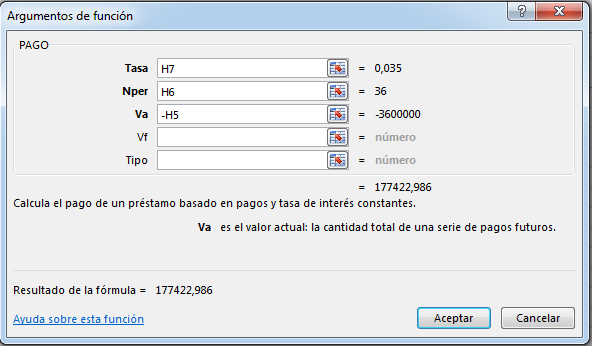
\includegraphics[height=5.4cm]{img/ch8/8_10.png}
\end{center}

=PAGO(H7;H6;-H5) con referencia en la hoja de Excel usada para el ejercicio.

\vspace{2mm}

\textbf{d}. Respuesta

\vspace{2mm}
La cuota ascenderá a  \$177.422,99.

\vspace{2mm}

\clearpage

\textbf{e}. Gráfica\\
\ \begin{center}
	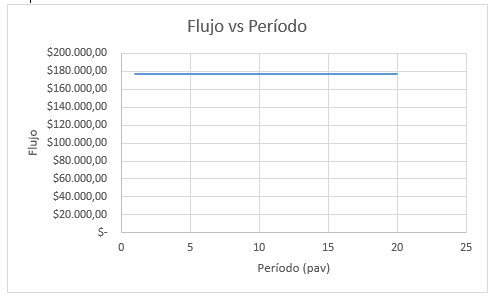
\includegraphics[height=5.4cm]{img/ch8/8_11.png}
\end{center}

\textbf{Ejemplo 7}\\

Tomado del Capítulo 4, ejercicio número 18
\\

Elaborar una tabla para amortizar la suma de \$3.000.000 en pagos trimestrales durante 15 meses con una tasa del 46\% nominal anual trimestre vencido

\vspace{2mm}

\textbf{Solución:}

\vspace{2mm}

\textbf{a}. Declaración de variables\\

	    $P=\$3.000.000,00$
	    \\
	    $	n=5 ptv 
	    \\
		i=11,5\% ptv
		\\
		$R=\$?$\\
	$	
\\
\textbf{b}.Tabla flujo de caja

    \begin{center}
        \begin{tabular}{|p{1cm}|p{2,5cm}|p{2,5cm}|p{2,5cm}|p{2,5cm}|p{2,5cm}|}
        \hline 
            \textbf{Per} & \textbf{Saldo Inicial} & \textbf{Intereses}& \textbf{Abono Capital} & \textbf{Cuota}& \textbf{Saldo Final}   \\ \hline                        

           
           
            0 & \$ &\$&\$&\$&\$3.000.000,00  \\ \hline
            1 & \$3.000.000,00  &\$345.000,00 &\$ 476.945,32 &\$821.945,32&\$2.523.054,68  \\ \hline
            2 & \$2.523.054,68 &\$290.151,29&\$531.794,03&\$821.945,32&\$1.991.260,66 \\ \hline
            3 & \$1.991.260,66 & \$228.994,98&\$592.950,34&\$ 821.945,32&\$ 1.398.310,32\\ \hline
            4 & \$1.398.310,32 &\$160.805,69&\$661.139,63&\$821.945,32&\$737.170,69  \\ \hline
            5 & \$ 737.170,69 &\$84.774,63&\$737.170,69&\$ 821.945,32&\$0,00 \\ \hline
             
\end{tabular}
\end{center}

\clearpage

\textbf{c}. Aplicación de funciones.
 \\
 
Se aplicará la función PAGO de la siguiente forma:     
 
 \begin{center}
	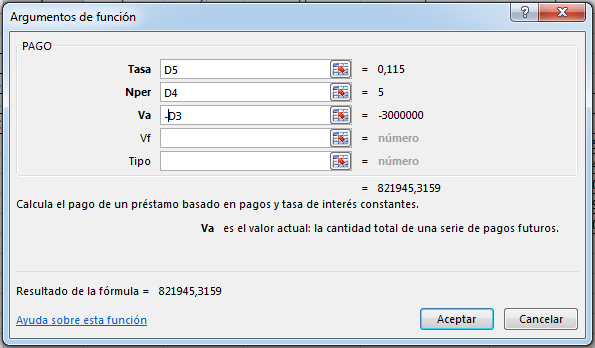
\includegraphics[height=5.4cm]{img/ch8/8_13.png}
\end{center}

=PAGO(D5;D4;-D3) con referencia en la hoja de Excel usada para el ejercicio.

\vspace{2mm}

\textbf{d}. Respuesta

\vspace{2mm}

El pago sera de \$821.945,32

\vspace{2mm}

\textbf{e}. Gráfica\\
\ \begin{center}
	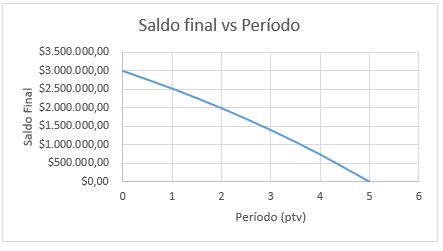
\includegraphics[height=5.4cm]{img/ch8/8_14.png}
\end{center}
\vspace{4mm}
\textbf{Ejemplo 8}\\

Tomado del Capítulo 5, ejercicio número 2

\vspace{2mm}

Hallar el valor presente de una renta perpetua vencida de \$10.000 mensuales, suponiendo un interés del 33\% nominal anual mes vencido.

\vspace{2mm}

\textbf{Solución:}
\vspace{2mm}


\textbf{a}. Declaración de variables

\vspace{2mm}


	    $R=\$1.000.000,00$
	    \\
	    $	n= \infty pmv 
	    \\
		i=2,75\% pmv
		\\
		$P=\$?$\\
		$	

\textbf{b}.Tabla flujo de caja

\vspace{2mm}

No tiene pues no hay sentido hacerlo por el número de períodos.

\vspace{2mm}

\textbf{c}. Aplicación de funciones.
 \\
 
Se aplicará la función VA de la siguiente forma:     
 
 \begin{center}
	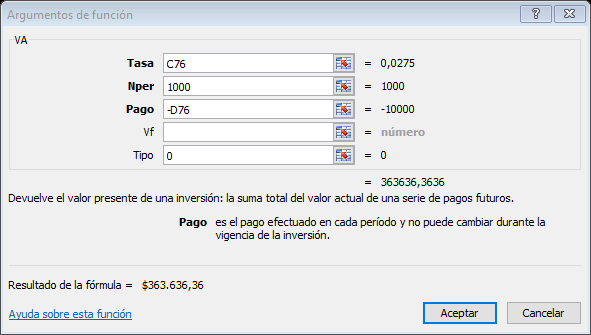
\includegraphics[height=5.4cm]{img/ch8/8_15.png}
\end{center}

=VA(C76;1000;-D76;;0) con referencia en la hoja de Excel usada para el ejercicio.

\vspace{2mm}

\textbf{d}. Respuesta

\vspace{2mm}

El valor presente es VP = \$363.636,36

\vspace{2mm}

\textbf{e}. Gráfica

\vspace{2mm}

No es necesaria una gráfica para este ejercicio.

\vspace{2mm}

\textbf{Ejemplo 9}

\vspace{2mm}

Tomado del Capítulo 6, ejercicio número 2

\vspace{2mm}

Hallar el valor presente con un interés del 5\% período año vencido de la siguiente gráfica:

 \begin{center}
	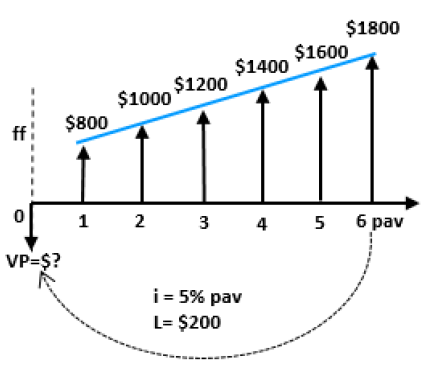
\includegraphics[height=5.4cm]{img/ch8/8_16.png}
\end{center}

\\\\
\textbf{Solución:}

\vspace{2mm}

\textbf{a}. Declaración de variables\\

	    $R=\$800,00$
	    \\
	    $L = 40\%$\\
	    $	n=6 pav 
	    \\
		i=3,5\% pav
		\\
		$P=\$?$\\
	$	
\\
\textbf{b}.Tabla flujo de caja
\\

\begin{spacing}{0.1}
\begin{center}
\begin{tabular}{ |p{3.5cm}| p{3cm}|}
\hline 

\begin{center}\textbf{Periodo (psv) } \end{center}  & \begin{center} \textbf{Flujo} \end{center}  \\ \hline

\begin{center} 0 \end{center}   &  \begin{center} - \end{center}\\\hline

\begin{center}1 \end{center}    &  \begin{center} \$800,00\end{center} \\ \hline

\begin{center}2 \end{center}    &  \begin{center} \$1.000,00\end{center} \\ \hline 

\begin{center}3 \end{center}    & \begin{center} \$1.200,00\end{center}  \\ \hline

\begin{center}4 \end{center}    & \begin{center} \$1.400,00 \end{center}  \\ \hline

\begin{center}5 \end{center}    & \begin{center} \$1.600,00\end{center}  \\ \hline

\begin{center}6 \end{center}    & \begin{center} \$1.800,00 \end{center}  \\ \hline
\end{tabular}
\end{center}
\end{spacing}
\\

\textbf{c}. Aplicación de funcioness.
 \\
 
Se aplicará la función VNA de la siguiente forma:     
 
 \begin{center}
	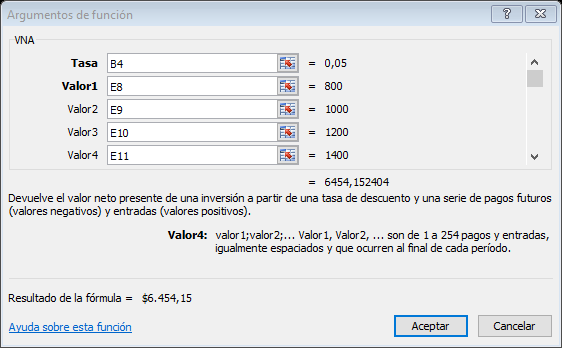
\includegraphics[height=5.4cm]{img/ch8/8_17.png}
\end{center}

=+VNA(B4;E8:E13) con referencia en la hoja de Excel usada para el ejercicio.

\vspace{2mm}

\textbf{d}. Respuesta

\vspace{2mm}

El valor presente es  \$6.454,15

\clearpage

\textbf{e}. Gráfica

\vspace{2mm}

\ \begin{center}
	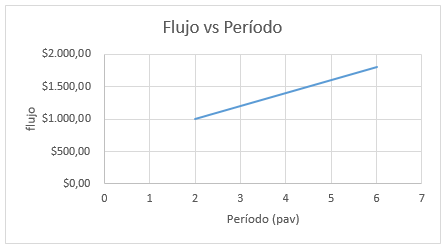
\includegraphics[height=5.4cm]{img/ch8/8_18.png}
\end{center}

\textbf{Ejemplo 10}\\

Tomado del Capítulo 6, ejercicio número 10
\\

¿Cuánto debe crecer linealmente una serie aritmética de 8 egresos, efectuados al final de cada período y cuyo primer egreso es de \$600 para que, puesta en valor presente, sea equivalente a una serie de 10 períodos que crecen geométricamente en un 25\% y cuyo primer egreso es de \$100? Suponga una tasa del 3\% período anual vencido.

\vspace{2mm}

\textbf{Solución:}

\vspace{2mm}

\textbf{a}. Declaración de variables\\

Gradiente Aritmético

	    $R=\$600,00$
	    \\
	    $	n=8 pav 
	    \\
		i=3,0\% pav
		\\
		L=\$?$\\
	
\\
Gradiente Geométrico

	    $R=\$100,00$
	    \\
	    $	n=10 pav 
	    \\
		i=3,0\% pav
		\\
		$G=25\%$\\
$

\clearpage

\textbf{b}.Tabla flujo de caja
\\

\item Gradiente Aritmético
\begin{spacing}{0.1}
\begin{center}
\begin{tabular}{ |p{3.5cm}| p{3cm}|}
\hline 
\begin{center}\textbf{Periodo (pav) } \end{center}  & \begin{center} \textbf{Flujo} \end{center}  \\ \hline

\begin{center}1 \end{center}    &  \begin{center} \$600,00\end{center} \\ \hline

\begin{center}2 \end{center}    &  \begin{center} \$600,00\end{center} \\ \hline 

\begin{center}3 \end{center}    & \begin{center} \$600,00 \end{center}  \\ \hline

\begin{center}4 \end{center}    & \begin{center} \$600,00\end{center}  \\ \hline

\begin{center}5 \end{center}    & \begin{center} \$600,00 \end{center}  \\ \hline

\begin{center}6 \end{center}    & \begin{center} \$600,00 \end{center}  \\ \hline

\begin{center}7 \end{center}    & \begin{center} \$600,00\end{center}  \\ \hline

\begin{center}8 \end{center}    & \begin{center} \$600,00 \end{center} \\ \hline

\begin{center}9 \end{center}    & \begin{center} \$600,00 \end{center} \\ \hline

\begin{center}10 \end{center}    & \begin{center} \$600,00 \end{center} \\ \hline

\end{tabular}
\end{center}
\end{spacing}
\\

\item Gradiente Geométrico
\begin{spacing}{0.1}
\begin{center}
\begin{tabular}{ |p{3.5cm}| p{3cm}|}
\hline 
\begin{center}\textbf{Periodo (psv) } \end{center}  & \begin{center} \textbf{Flujo} \end{center}  \\ \hline

\begin{center}1 \end{center}    &  \begin{center} \$100,00\end{center} \\ \hline

\begin{center}2 \end{center}    &  \begin{center} \$125,00\end{center} \\ \hline 

\begin{center}3 \end{center}    & \begin{center} \$156,25 \end{center}  \\ \hline

\begin{center}4 \end{center}    & \begin{center} \$195,31\end{center}  \\ \hline

\begin{center}5 \end{center}    & \begin{center} \$244,14 \end{center}  \\ \hline

\begin{center}6 \end{center}    & \begin{center} \$305,18 \end{center}  \\ \hline

\begin{center}7 \end{center}    & \begin{center} \$381,47\end{center}  \\ \hline

\begin{center}8 \end{center}    & \begin{center} \$476,84 \end{center} \\ \hline

\begin{center}9 \end{center}    & \begin{center} \$596,05 \end{center} \\ \hline

\begin{center}10 \end{center}    & \begin{center} \$745,06 \end{center} \\ \hline

\end{tabular}
\end{center}
\end{spacing}
\\

\clearpage

\textbf{c}. Aplicación de funciones.
 \\
 
Para el gradiente Aritmético se aplicará la función  valor presente VNA de la siguiente forma:     
 
 \begin{center}
	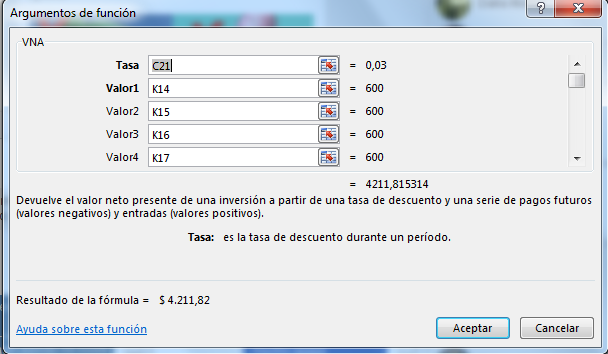
\includegraphics[height=5.4cm]{img/ch8/8_19.png}
\end{center}

=VNA(B36;F25;F26;F27;F28;F29;F30;F31;F32) con referencia en la hoja de Excel usada para el ejercicio encontrando que VP = \$4.211,82.
\\ 
 
Para el gradiente Geométrico se aplicará la función  valor presente VNA de la siguiente forma:     
 
 \begin{center}
	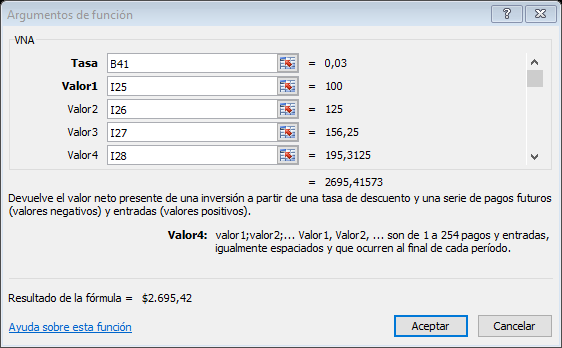
\includegraphics[height=5.4cm]{img/ch8/8_20.png}
\end{center}

=VNA(B41;I25;I26;I27;I28;I29;I30;I31;I32;I33;I34) con referencia en la hoja de Excel usada para el ejercicio encontrando que VP = \$2.695,42.

\vspace{2mm}

Luego usando la función ‘’Buscar objetivo’’, poniendo a variar L hacemos que el VP de ambos gradientes sea el mismo.

\begin{center}
	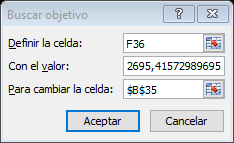
\includegraphics[height=5.4cm]{img/ch8/8_21.png}
\end{center}
\\ 
\textbf{d}. Respuesta\\

El gradiente aritmético debe crecer L = -\$64,5809 lo que significa que el gradiente es decreciente.

\vspace{2mm}

\item Gradiente Aritmético
\begin{spacing}{0.1}
\begin{center}
\begin{tabular}{ |p{3.5cm}| p{3cm}|}
\hline 
\begin{center}\textbf{Periodo (pav) } \end{center}  & \begin{center} \textbf{Flujo} \end{center}  \\ \hline

\begin{center}1 \end{center}    &  \begin{center} \$600,00\end{center} \\ \hline

\begin{center}2 \end{center}    &  \begin{center} \$535,42\end{center} \\ \hline 

\begin{center}3 \end{center}    & \begin{center} \$470,84 \end{center}  \\ \hline

\begin{center}4 \end{center}    & \begin{center} \$406,26\end{center}  \\ \hline

\begin{center}5 \end{center}    & \begin{center} \$341,68 \end{center}  \\ \hline

\begin{center}6 \end{center}    & \begin{center} \$277,10 \end{center}  \\ \hline

\begin{center}7 \end{center}    & \begin{center} \$212,51\end{center}  \\ \hline

\begin{center}8 \end{center}    & \begin{center} \$147,93 \end{center} \\ \hline
\end{tabular}
\end{center}
\end{spacing}
\\
\\\\
\textbf{e}. Gráfica\\
\ \begin{center}
	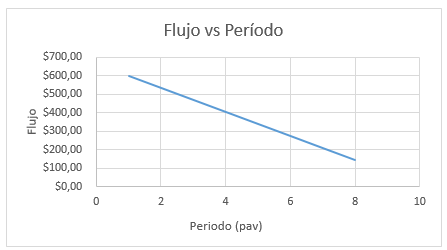
\includegraphics[height=5.4cm]{img/ch8/8_22.png}
\end{center}
\textbf{Ejemplo 11}\\

Tomado del Capítulo 6, ejercicio número 2
\\

Hallar el valor presente de 15 pagos que decrecen linealmente en \$400, si el primer pago es de \$5.000 y la tasa efectiva es del 4\% período año vencido.

\vspace{2mm}

\textbf{Solución:}

\textbf{a}. Declaración de variables\\


	    $R=\$5.400,00$
	    \\
	    $	n=15 pav$ 
	    \\
		$i=4,0\% pav$
		\\
		$L=\$400,00$\\
		$VP=\$?$

\textbf{b}.Tabla flujo de caja

\begin{spacing}{0.1}
\begin{center}
\begin{tabular}{ |p{3.5cm}| p{3cm}|}
\hline 
\begin{center}\textbf{Periodo (pav) } \end{center}  & \begin{center} \textbf{Flujo} \end{center}  \\ \hline

\begin{center}0 \end{center}    &  \begin{center} \end{center} \\ \hline

\begin{center}1 \end{center}    &  \begin{center} \$400,00\end{center} \\ \hline

\begin{center}2 \end{center}    &  \begin{center} \$800,00\end{center} \\ \hline 

\begin{center}3 \end{center}    & \begin{center} \$1.200,00 \end{center}  \\ \hline

\begin{center}4 \end{center}    & \begin{center} \$1.600,00\end{center}  \\ \hline

\begin{center}5 \end{center}    & \begin{center} \$2.000,00 \end{center}  \\ \hline

\begin{center}6 \end{center}    & \begin{center} \$2.400,00 \end{center}  \\ \hline

\begin{center}7 \end{center}    & \begin{center} \$2.800,00\end{center}  \\ \hline

\begin{center}8 \end{center}    & \begin{center} \$3.200,00 \end{center} \\ \hline

\begin{center}9 \end{center}    & \begin{center} \$3.600,00 \end{center} \\ \hline

\begin{center}10 \end{center}    & \begin{center} \$4.000,00 \end{center} \\ \hline

\begin{center}11 \end{center}    & \begin{center} \$4.400,00 \end{center} \\ \hline

\begin{center}12 \end{center}    & \begin{center} \$4.800,00 \end{center} \\ \hline

\begin{center}13 \end{center}    & \begin{center} \$5.200,00 \end{center} \\ \hline

\begin{center}14 \end{center}    & \begin{center} \$5.600,00 \end{center} \\ \hline

\begin{center}15 \end{center}    & \begin{center} \$6.000,00 \end{center} \\ \hline
\end{tabular}
\end{center}
\end{spacing}

\vspace{2mm}
\vspace{2mm}

\textbf{c}. Aplicación de funciones.
 \\
 
Se aplicará la función  valor presente VNA de la siguiente forma:     
 
 \begin{center}
	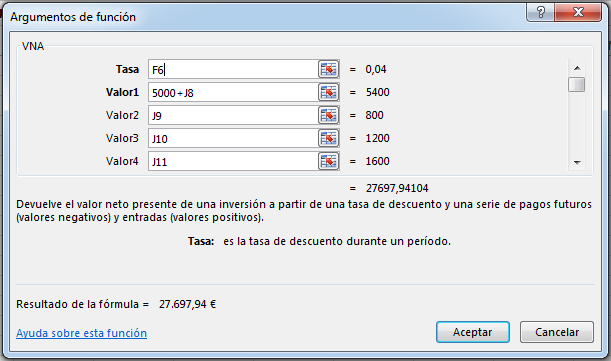
\includegraphics[height=5.4cm]{img/ch8/8_23.png}
\end{center}
=VNA(F6;J8;J9;J10;J11;J12;J13;J14;J15;J16;J17;J18;J19;J20;J21;J22) con referencia en la hoja de Excel usada para el ejercicio.
\\ 
 
\textbf{d}. Respuesta\\

El valor presente es VP = \$27.697,9410

\vspace{2mm}

\textbf{e}. Gráfica\\
\ \begin{center}
	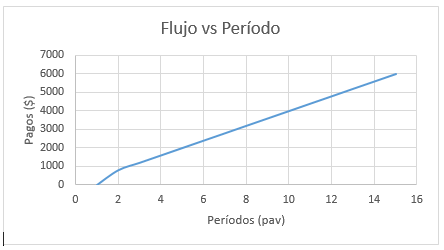
\includegraphics[height=5.4cm]{img/ch8/8_24.png}
\end{center}

\textbf{Ejemplo 12}\\

Ejemplo del capitulo
\\

Elaborar una tabla que muestre la amortización de \$3.000.000 mediante pagos mensuales durante 3,5 años con una tasa del 3\% período mes vencido.

\vspace{2mm}

\textbf{Solución:}

\textbf{a}. Declaración de variables\\


	    $VP=\$3.000.000,00$
	    \\
	    $	n=42 pmv$ 
	    \\
		$i=3,0\% pmv$
		\\
				$R=\$?$

\clearpage

\textbf{b}.Tabla flujo de caja
\begin{spacing}{1.1}
    \begin{center}
        \begin{tabular}{|p{1cm}|p{2,5cm}|p{2,5cm}|p{2,5cm}|p{2,5cm}|p{2,5cm}|}
        \hline 
            \textbf{Per} & \textbf{Saldo Inicial} & \textbf{Intereses}& \textbf{Abono Capital} & \textbf{Cuota}& \textbf{Saldo Final}   \\ \hline                        

           
           
            0 & \$3.000.000,00 &\$&\$&\$&\$3.000.000,00  \\ \hline
            1 & \$3.000.000,00  &\$90.000,00 & -\$ 90.000,00 &\$0,00&\$ 3.090.000,00  \\ \hline
            2 & \$ 3.090.000,00 &\$92.700,00&-\$92.700,00&\$0,00&\$3.182.700,00 \\ \hline
            3 & \$3.182.700,00 & \$95.481,00&-\$95.481,00&\$ 0,00&\$ 3.278.181,00\\ \hline
            4 & \$3.278.181,00 &\$98.345,43&-\$98.345,43&\$0,00&\$3.376.526,43 \\ \hline
            5 & \$3.376.526,43 &\$101.295,79&-\$101.295,79&\$0,00&\$3.477.822,22 \\ \hline
            6 & \$3.477.822,22 &\$104.334,67&-\$104.334,67&\$0,00&\$ 3.582.156,89  \\ \hline
            7 & \$ 3.582.156,89  &\$107.464,71 & -\$ 107.464,71 &\$0,00&\$ 3.689.621,60  \\ \hline
            8 & \$ 3.689.621,60 &\$110.688,65&-\$110.688,65&\$0,00&\$ 3.800.310,24 \\ \hline
            9 & \$ 3.800.310,24 & \$114.009,31&-\$114.009,31&\$ 0,00&\$ 3.914.319,55\\ \hline
            10 & \$3.914.319,55 &\$117.429,59&-\$117.429,59&\$0,00&\$4.031.749,14 \\ \hline
            11& \$4.031.749,14 &\$101.295,79&-\$101.295,79&\$0,00&\$0,00 \\ \hline
            . & \$ . &\$ .&\$ .&\$. &\$. \\ \hline
            . & \$ . &\$ .&\$ .&\$. &\$. \\ \hline
            . & \$ . &\$ .&\$ .&\$. &\$. \\ \hline
            . & \$ . &\$ .&\$ .&\$. &\$. \\ \hline
            39 & \$9.224.350,43 &\$276.730,51&-\$276.730,51&\$0,00&\$9.501.080,95  \\ \hline
            40 & \$9.501.080,95 &\$285.032,43&-\$285.032,43&\$0,00&\$9.786.113,38 \\ \hline
            41 & \$9.786.113,38 &\$293.583,40&-\$293.583,40&\$0,00&\$10.079.696,78  \\ \hline
            42 & \$10.079.696,78 &\$302.390,90&-\$302.390,90&\$0,00&\$10.382.087,68 \\ \hline
             
\end{tabular}
\end{center}
\end{spacing}
\vspace{2mm}

\textbf{c}. Aplicación de funciones.
 \\
 
Se aplicará la función   Buscar  objetivo de la siguiente forma:     
 
 \begin{center}
	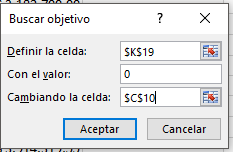
\includegraphics[height=5.4cm]{img/ch8/8_25.png}
\end{center}
\\ 
 
\textbf{d}. Respuesta\\

De esta forma se obtiene el valor de \$126.575,02 para la cuota.

\clearpage

\textbf{e}. Gráfica\\
\ \begin{center}
	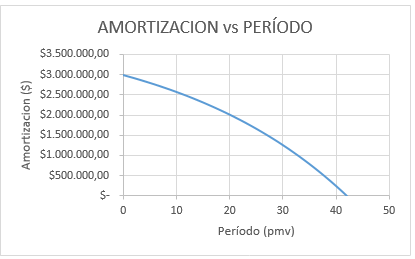
\includegraphics[height=5.4cm]{img/ch8/8_26.png}
\end{center}


%----------------------------------------------------------------------------------------


%----------------------------------------------------------------------------------------

%\part{Parte Dos}
    
%----------------------------------------------------------------------------------------
%	CHAPTER 3
%----------------------------------------------------------------------------------------

%\chapterimage{ima2} % Chapter heading image


%Anexos
%\chapter*{Anexos}
%\addcontentsline{toc}{chapter}{\textcolor{ocre}{Anexos}}




%----------------

%----------------------------------------------------------------------------------------
%	BIBLIOGRAPHY
%----------------------------------------------------------------------------------------

%\chapter*{Bibliografía}
%\addcontentsline{toc}{chapter}{\textcolor{ocre}{Bibliografía}}
%\section*{Books}
%\addcontentsline{toc}{section}{Books}
%\printbibliography[heading=bibempty,type=book]



%----------------------------------------------------------------------------------------
%	INDEX
%----------------------------------------------------------------------------------------

\cleardoublepage
\phantomsection
\setlength{\columnsep}{0.75cm}
\printindex

%----------------------------------------------------------------------------------------

